\documentclass[sigconf,10pt]{acmart}

%\usepackage[•]{•}{microtype}

\usepackage{booktabs} % For formal tables
%\usepackage[moderate]{savetrees}
\settopmatter{printacmref=false}
% Copyright
%\setcopyright{none}
%\setcopyright{acmcopyright}
%\setcopyright{acmlicensed}
\setcopyright{rightsretained}
%\setcopyright{usgov}
%\setcopyright{usgovmixed}
%\setcopyright{cagov}
%\setcopyright{cagovmixed}
\newcommand{\minihead}[1]{{\vspace{.5em}\noindent\textbf{#1} }}
\newcommand{\red}[1]{{\color{red}#1}}
\newcommand{\mvar}{\red{d}}
\newcommand{\dvar}{\red{n}}

\newcommand\code[1]{\lstinline$#1$}




\usepackage{enumitem}


\usepackage{algorithm}
\usepackage[noend]{algpseudocode}
\algdef{SE}[DOWHILE]{Do}{doWhile}{\algorithmicdo}[1]{\algorithmicwhile\ #1}%

\theoremstyle{problem}
\newtheorem{problem}{Problem}[section]



% DOI
%\acmDOI{10.475/123_4}

% ISBN
%\acmISBN{123-4567-24-567/08/06}

%Conference
\acmConference[DEEM'19]{DEEM}{June 2019}{Amsterdam, The Netherlands}
\acmYear{2019}



\begin{document}
\title{DROP: Optimizing Stochastic Dimensionality \\ Reduction \red{via Workload-Aware Progressive Sampling}}


\author{Sahaana Suri, Peter Bailis}
\affiliation{
  \institution{Stanford University}
}


\maketitle


\begin{abstract}
Dimensionality reduction is crucial to a number of data analytics workflows, such as anomaly detection, classification, and predictive analysis, and has been extensively studied in a variety of domains, including statistics, signal processing and data mining. Recently, there has been an increase in the amount of data generated from automated sensors, devices and processes, collectively, the Internet of Things (IoT). It is becoming increasingly important for data analytics techniques to scale to these immense volumes of IoT, often time-series, data to extract value from them in a timely fashion. 

Analysis of various dimensionality reduction techniques reveals that given an accuracy bound on pairwise distance preservation, Principal Component Analysis (PCA) outperforms most other techniques with respect to accuracy, but is often orders of magnitude slower than other techniques. However, by exploiting the structure present in automatically generated IoT and time series data, we develop a new, sampling-based technique for automatically and efficiently finding the optimal low-dimensional basis for a given time-series and/or IoT dataset---DROP (Dimensionality Reduction OPtimizer). DROP iteratively subsamples the dataset and searches for an $\epsilon$-distance-preserving transformation.
For time-series and IoT data with limited variance, this allows DROP to uncover the optimal basis in running time that is \textit{independent} of the actual dataset size and \textit{without} requiring the user to specify the intrinsic dimensionality of the dataset a priori; instead, DROP discovers it. This provides order of magnitude speedups over na{\"i}ve PCA and blah blah.  


 \end{abstract}


\section{Introduction}
\label{sec:intro}

Continued, rapid growth in high-dimensional data from automated data sources~\cite{plato,macrobase-cidr} poses a scalability challenge for machine learning (ML) pipelines.
In exchange for a preprocessing cost, dimensionality reduction (DR) techniques can accelerate ML training and inference/query execution (as a result of smaller data points), improving overall pipeline runtime (see Figure~\ref{fig:pipeline}) while preserving accuracy~\cite{keogh-indexing,local-dr,decade,gemini}.

Principal Component Analysis (PCA) is often the DR method of choice for practitioners with respect to transformation quality and downstream accuracy~\cite{jolbook}. However, na\"{i}ve implementations of PCA are data and workload-independent, and scale poorly with dimensionality, resulting in preprocessing times that exceed the downstream runtime benefit of DR. As a result, practitioners are willing to sacrifice quality (i.e., size of lower dimension representation at a given accuracy) for runtime, and use alternative DR methods~\cite{keogh-study}. 


Sample-based, stochastic PCA algorithms~\cite{shamir,re-new} are a scalable alternative to classical PCA.
However, the amount of sampling required is highly data-dependent.
If we sample too many data points, then the runtime overhead of PCA in an end-to-end analytics workload could outweigh the statistical benefits.
If we fail to sample enough data points, then PCA could fail to deliver a sufficiently high-quality reduction and compromise the runtime and/or accuracy of downstream analytics.
This raises a critical question: can we develop a data and workload-dependent means of efficiently and accurately determining the sampling rate that minimizes end-to-end workload runtime while ensuring high accuracy?

\begin{figure}
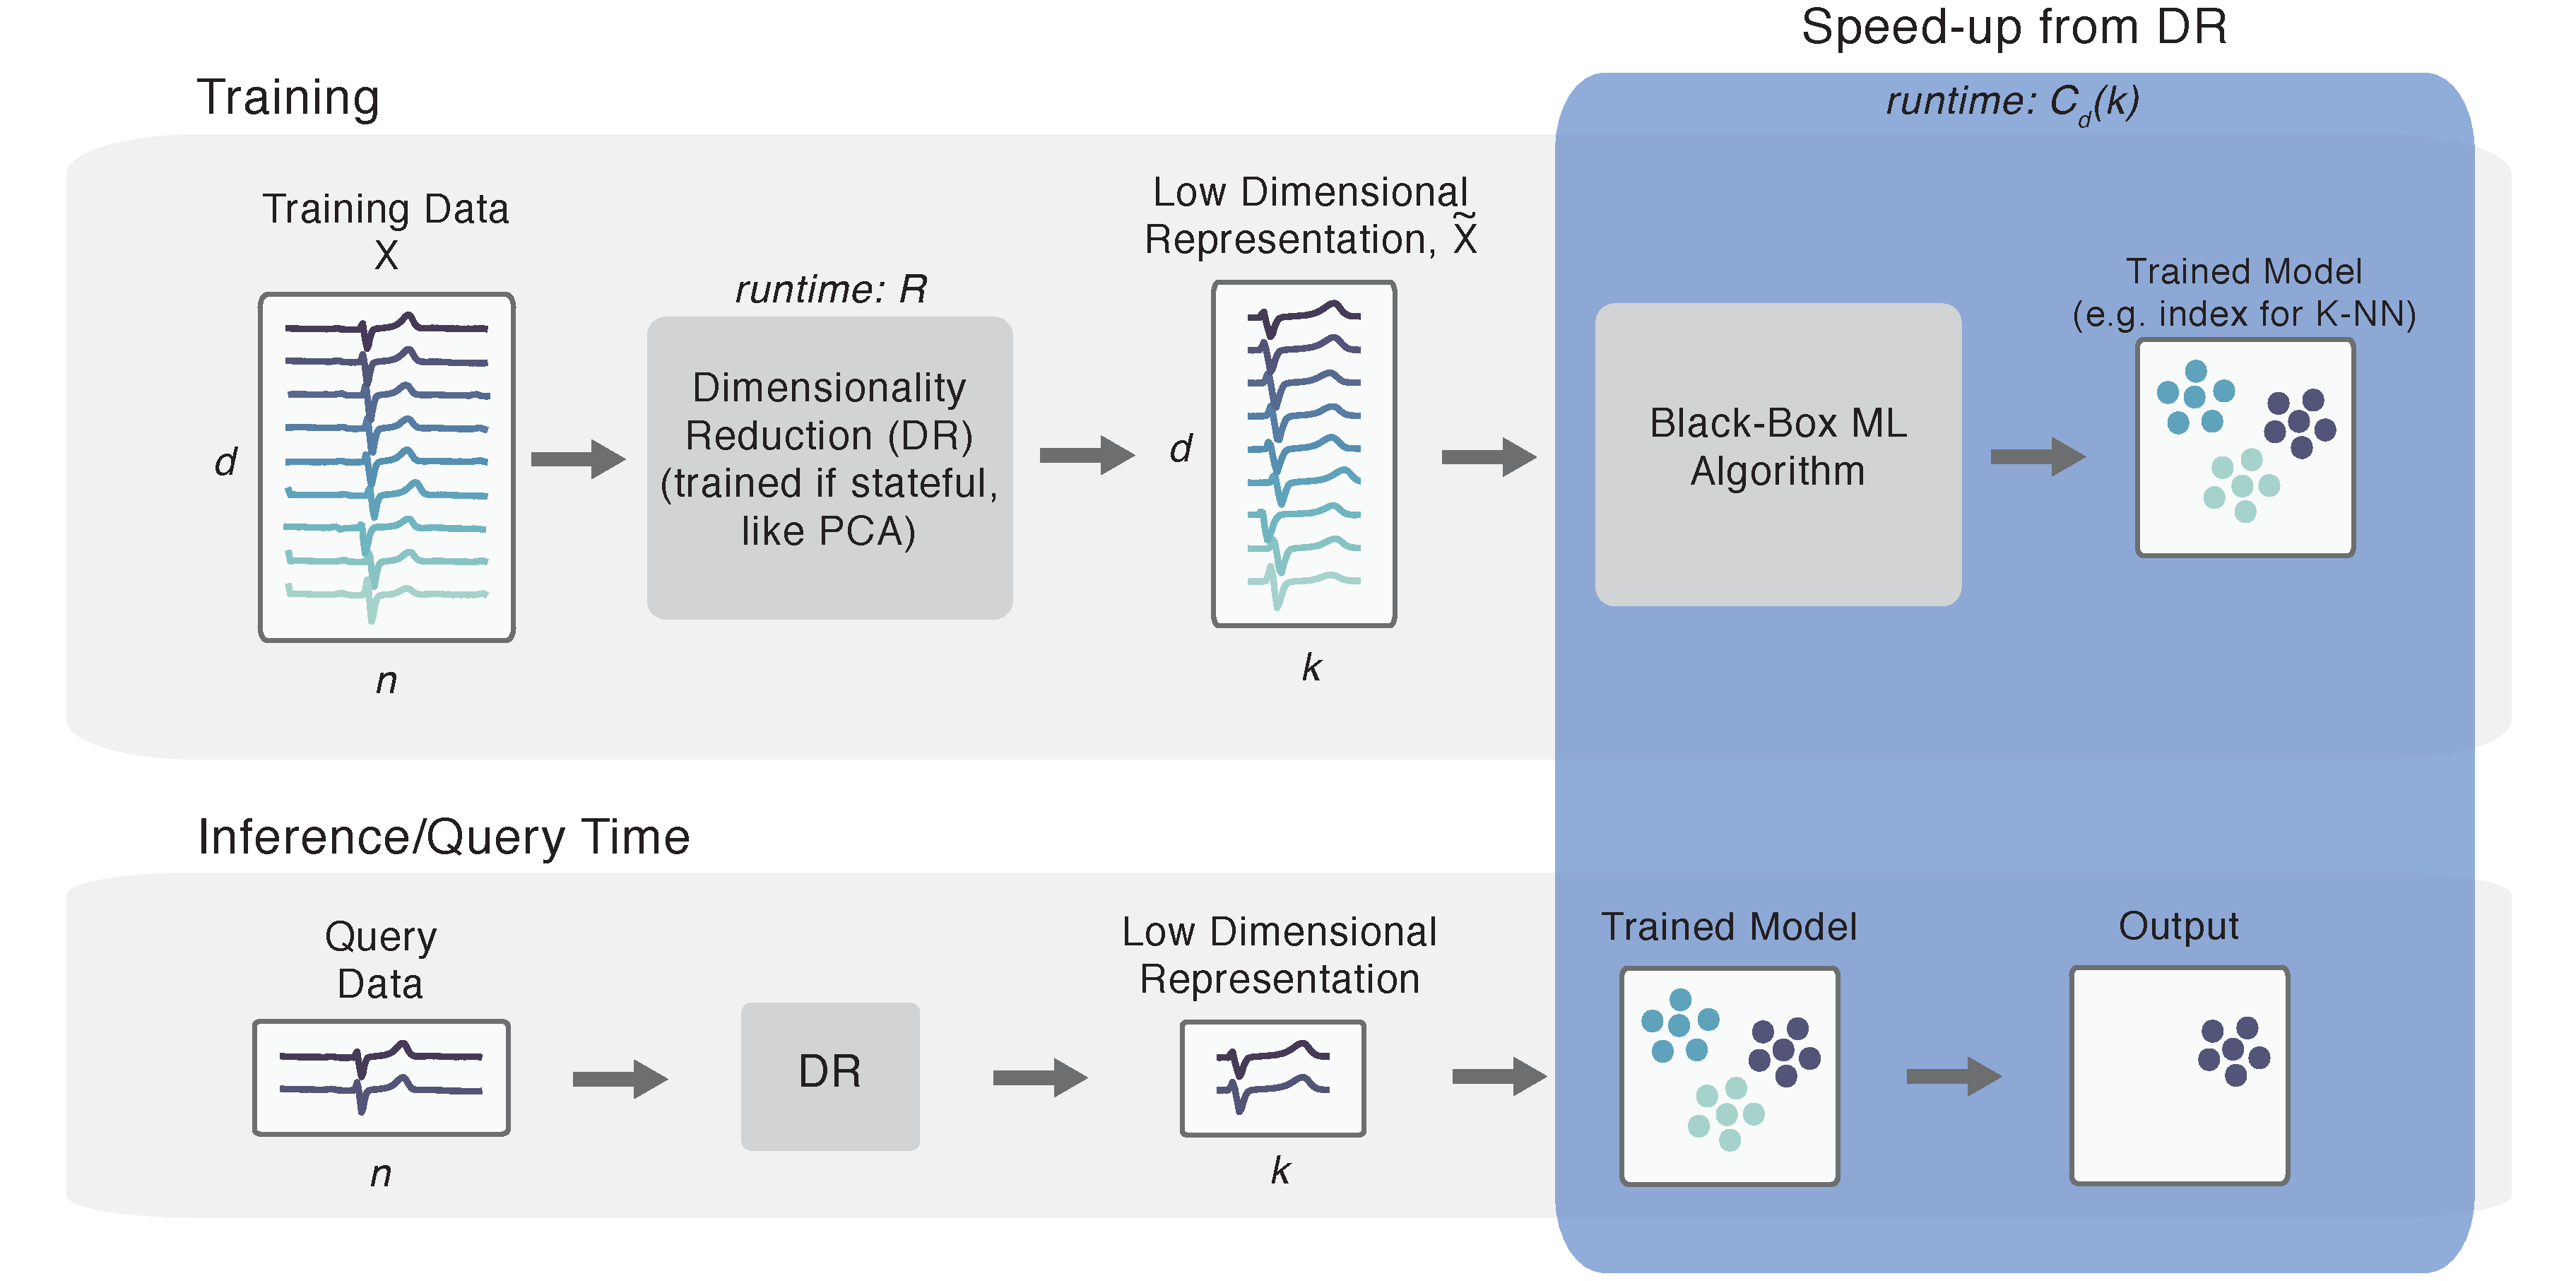
\includegraphics[width=\linewidth]{figs/pipeline.pdf}
\caption[]{Sample machine learning pipeline with dimensionality reduction. Spending time on DR provides downstream runtime speed-ups.}
\label{fig:pipeline}
\end{figure}


To this end, we develop DROP, a system that performs whole-workload runtime optimization by dynamically identifying the amount of sampling required for stochastic PCA.
DROP takes a high-dimensional dataset,\footnote{Our primary focus \red{for performance evaluation is a case study on time series similarity search,} given the amount of study in the database community~\cite{keogh-study} and the resurgence of interest in time series analytics systems~\cite{macrobase,macrobase-cidr,trill-signal}. We provide a preliminary generalizability analysis in Section~\ref{sec:experiments}.}  property to preserve (e.g., pairwise Euclidean distance to 5\%), and optional runtime model expressing downstream workload performance as a function of dimensionality (e.g., for k-Nearest Neighbors [k-NN], runtime is linear in dimensionality). 
DROP returns a low-dimensional transformation for the input using as few samples as needed to minimize the projected overall workload runtime while satisfying quality constraints.

\begin{figure}
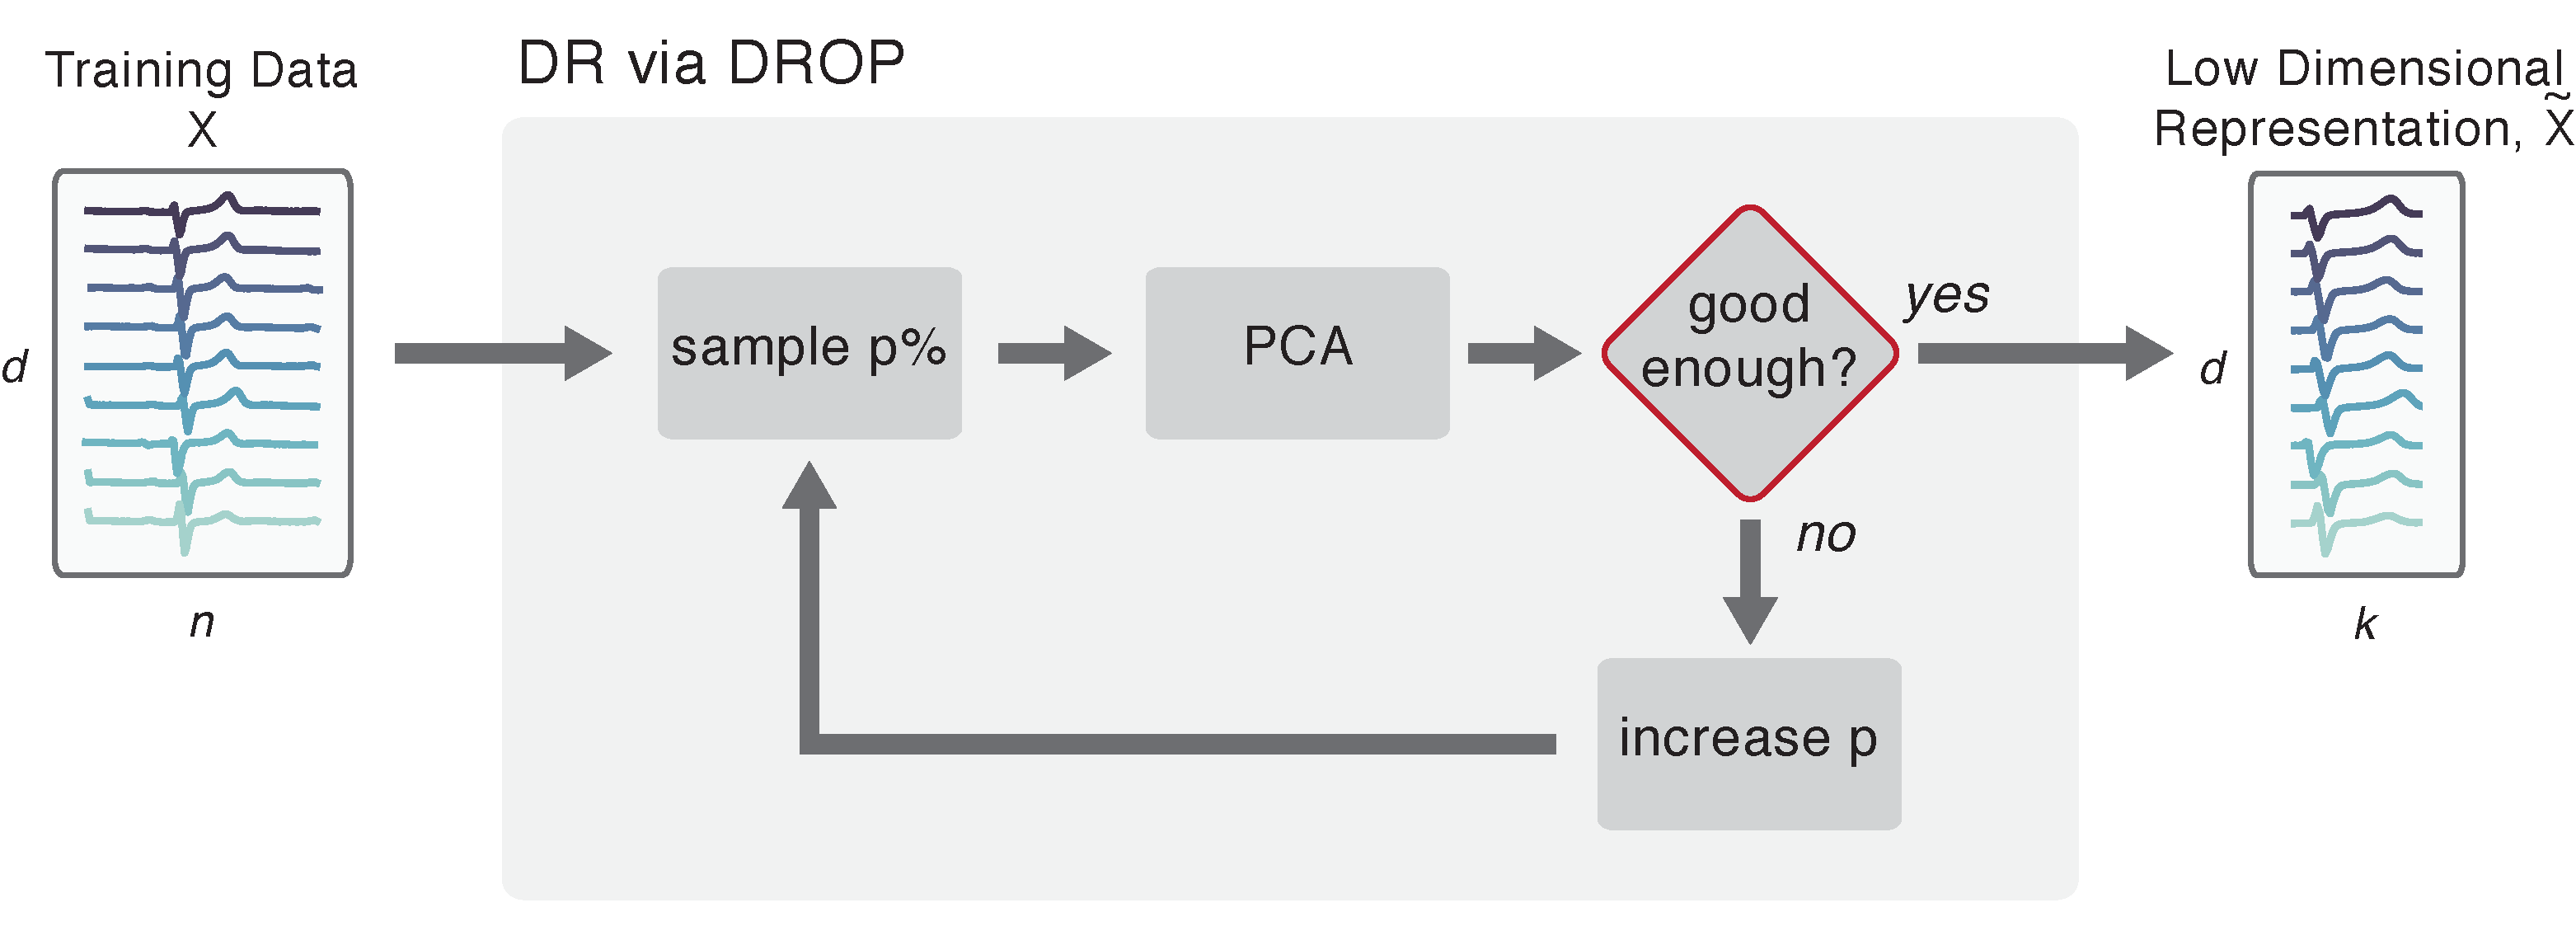
\includegraphics[width=\linewidth]{figs/basic.pdf}
\caption[]{DROP is a DR operator compatible with standard ML pipelines. The challenge DROP solves is when to stop training---is the low dimensional representation trained via a data sample ``good enough"?}
\label{fig:basic}
\end{figure}

%%%%%%

To achieve this functionality, DROP addresses the question of how much to sample the input dataset by adapting techniques from the approximate query processing literature: data-dependent progressive sampling and online progress estimation at runtime.  
DROP performs PCA on a small sample to obtain a candidate transformation, then progressively increases the number of samples until termination (see Figure~\ref{fig:basic}). 
To identify the termination point that minimizes the overall runtime, DROP must overcome three challenges:

First, given the results of PCA on a data sample, DROP must \emph{evaluate the quality} of the current candidate transformation.
Popular analytics and data mining tasks often require approximate preservation of metrics such as average pairwise distances between data points~\cite{time-series-dm,dm-book}, which are costly to compute.
Thus, DROP adapts confidence intervals (either via closed-form or, if unavailable, via bootstrapping) for fast estimation of the input metric to preserve.


Second, DROP must \emph{estimate the marginal benefit of sampling additional datapoints} for another iteration.
When running PCA on a series of progressively larger samples, later samples will incur higher computational cost but may return lower-dimensional transformations. 
To navigate this trade-off between end-to-end runtime and transformation quality, DROP uses the results obtained from previous iterations to build a predictive performance model for future iterations.


Finally, given the current quality and expected marginal benefit of the next iteration, DROP must \emph{optimize end-to-end runtime}.
While an application-agnostic approach would iterate until successive iterations yield no benefit to quality, many analytics operators such as k-Nearest Neighbors are tolerant of error~\cite{gemini}, so it is frequently advantageous to trade a slightly higher-dimensional basis for faster pre-processing (DR).
To address this challenge, the system performs workload-specific optimization to minimize the expected runtime of the complete end-to-end analytics pipeline.


\begin{comment}

PCA is guaranteed to find the optimal linear transformation with respect to $\mathcal{L}_2$ reconstruction error, popular analytics and data mining tasks (e.g., k-NN~\cite{time-series-dm}, k-means~\cite{dm-book},  kernel density estimation~\cite{wand}) instead require approximate preservation of metrics such as average pairwise distances between data points.
To overcome this challenge, DROP adapts confidence intervals (either via closed-form or, if unavailable, via bootstrapping) for fast estimation of the input metric to preserve.


Since PCA is guaranteed to find the optimal linear transformation with respect to $\mathcal{L}_2$ reconstruction error, we could consider estimating the transformation quality using this quantity.
However, many popular analytics and data mining tasks (e.g., k-NN~\cite{time-series-dm}, k-Means~\cite{dm-book},  Kernel Density Estimation~\cite{wand}) do not use reconstruction error, and instead require approximate preservation of metrics such as average pairwise distances between data points.
A transformation that minimizes reconstruction error is not guaranteed to preserve the pairwise distance by the same amount.
Moreover, na\"ively computing pairwise distances as required for k-NN is prohibitively expensive, with quadratic runtime.
To overcome this challenge, the system adapts an approach pioneered for deterministic queries in the context of online aggregation: treat quality metrics as aggregation functions and use confidence intervals (either via closed-form or, if unavailable, via bootstrapping) for fast estimation.
This approach allows DROP to accurately estimate representation quality while avoiding the overhead of exact computation.

Second, DROP must \emph{estimate the marginal benefit of continuing to sample} for another iteration.
When running PCA on a series of progressively larger samples, later samples will incur higher computational cost but may in turn return lower-dimensional transformations. 
To navigate this trade-off between end-to-end runtime and transformation quality, the system performs online progress estimation, using the results obtained from previous iterations to build a predictive performance model for future iterations.
%This allows DROP to quantify the expected benefit of continued sampling.

Finally, given the current quality and expected marginal benefit of the next iteration, DROP must \emph{optimize end-to-end runtime} to determine whether to terminate.  
The system must evaluate if the expected marginal benefit to dimensionality arising from continuing to iterate would reduce total runtime.
While an application-agnostic approach would iterate until successive iterations yield no benefit to quality, many analytics operators such as k-Nearest Neighbors are tolerant of error~\cite{gemini}, so it is frequently advantageous to trade a slightly higher-dimensional basis for faster pre-processing (DR).
To address this challenge, the system performs workload-specific optimization to minimize the expected runtime of the complete end-to-end analytics pipeline.
\end{comment}

\begin{comment}
A simple, application-agnostic approach to addressing this problem would iterate until until successive iterations yield no benefit to quality, thus converging to the lowest-dimensional metric-preserving transformation.
However, as we have hinted, many time-series analytics operators such as k-Nearest Neighbors are tolerant of approximation error~\cite{gemini}, and it is frequently advantageous to trade a slightly higher-dimensional basis for faster pre-processing. In these settings, running to convergence is often wasteful.
To address this challenge, DROP performs a workload-specific optimization, utilizing a provided (or profiled) application-specific runtime model and performs online optimization  to minimize the expected runtime of the complete end-to-end analytics pipeline.
\end{comment} 

We view DROP as a pragmatic combination of recent theoretical advances in dimensionality reduction and classic techniques from approximate query processing, and a useful system for performing end-to-end workflow optimization.
We make the following contributions in this work:
\begin{itemize}

\item We show the data sample required to perform accuracy-achieving PCA is often small (as little as $1\%$), and data-dependent sampling can enable \red{$91\times$} speedup compared to PCA via singular value decomposition (SVD). 
%We show that as little as $2\%$ of time series data suffices to preserve pairwise distances within $2\%$, providing a $55.6\times$ reduction in dimension.
  %this came from the oracle numbers--used 0.002 and then looked at table
  
\item We propose DROP, an online optimizer for DR that uses information about downstream analytics tasks to perform efficient stochastic PCA.
%. DROP uses information about downstream analytics tasks to utilize as few samples as required to minimize the overall workload runtime, while satisfying constraints on the reduction quality.

\item We present techniques based on progressive sampling, approximate query processing, online progress estimation, and cost based optimization to enable up to \red{$5\times$} faster end-to-end execution over PCA via SVD.% and up to $3\times$ faster end-to-end execution than alternative techniques on real analytics pipelines.
\end{itemize}




\section{Problem Statement and DR Background}
\label{sec:background}

We provide background on dimensionality reduction (DR) and revisit a widely cited empirical comparison of DR techniques from VLDB 2008~\cite{keogh-study} \red{that we use as a case study.
We show} that Principal Component Analysis (PCA) can outperform classic techniques, but at a high computational cost.

\subsection{Dimensionality Reduction}
\label{sec:defs}

%As time series grow larger and richer with respect to the number of metrics and metadata collected (e.g., as sensor fidelity and sampling rates increase), DR becomes important in their analysis~\cite{macrobase}.
DR refers to finding a low-dimensional representation of a dataset that preserves properties of interest, such as data point similarity~\cite{dr-survey1,dr-survey2}.
Formally, consider $\mvar$ data vectors of length $\dvar$, $x_i \in \mathbb{R}^\dvar$, with $\mvar > \dvar$. 
We can represent this as a dataset matrix $X \in \mathbb{R}^{\mvar \times \dvar}$, where each row $i$ corresponds to vector $x_i$.  
DR computes a transformation function ($T: \mathbb{R}^\dvar \rightarrow \mathbb{R}^k$) that maps each $x_i$ to a new basis as $\tilde{x}_i \in \mathbb{R}^k$ where $k \leq \dvar$, resulting in a new data matrix $T(X) = \tilde{X} \in \mathbb{R}^{\mvar \times k}$ that preserves some metric of interest.  

DR techniques optimize for various metrics. 
%For instance, DR via Locality Sensitive Hashing~\cite{lsh} can preserve distance metrics such as Hamming distance and Jaccard similarity, and
In similarity search, for instance, a popular metric to preserve is the average Euclidean distance between pairs of points, which the literature refers to as \emph{tightness of lower bounds} ($TLB$)~\cite{gemini,keogh-study}.


\subsubsection*{Principal Component Analysis (PCA)}
\label{sec:pca}
PCA is a linear DR technique that identifies a new orthogonal basis for a dataset that captures its directions of highest variance.
Of all linear transformations, this basis minimizes reconstruction error in a mean square sense. 
Classically implemented PCA uses a Singular Value Decomposition (SVD) routine~\cite{trefethen}.
%, which computes the matrix decomposition $X = U \Sigma V^\intercal$.  
%Given a data matrix $X$, PCA via SVD forms the PCA transformation matrix $T:\mathbb{R}^\dvar \rightarrow \mathbb{R}^k$ by first subtracting each column in $X$ by the column's mean to obtain $C_X$ ($\mathbf{1}^\intercal C_X = \mathbf{0}$). 
%The first $k$ right singular vectors of $C_X$ (first $k$ columns of $V$ from the SVD of $C_X$) comprise $T$.  

\begin{comment} 
\begin{algorithm}
\begin{algorithmic}[1]
\Statex \textbf{Inputs:}  
\Statex $X \in \mathbb{R}^{m_1 \times d}$: training data matrix 
\Statex $Y \in \mathbb{R}^{m_2 \times d}$: data matrix to transform 
\Statex $k \in \mathbb{Z}_+$: desired dimensionality of transformed data
\Statex \textsc{SVD-T}: any truncated SVD algorithm  
\Statex
\Statex \hrule
\Function{fit}{$X$}:
	\State $\bar{X} = \text{columnMeans}(X)$
	\State $C_X = X - \bar{X}$
		\Comment{$C_X \in \mathbb{R}^{m_1 \times d}$}
	\State \textbf{Store: } $\bar{X}, C_A$
\EndFunction

\Function{transform}{$Y, k, $ \textsc{SVD-T}}:
	\State $U, \Sigma, V^T$ = \textsc{SVD-T}$(C_X, k)$
		\Comment{$V \in \mathbb{R}^{d \times k}$}
	\State $C_Y = Y - \bar{X}$
		\Comment{$C_Y \in \mathbb{R}^{m_2 \times d}$} 
	\State \textbf{Store: } $T = V$ 
			\Comment{Cache for repeated use} \\
	\Return $C_YT$
		%\Comment{$C_BV \in \mathbb{R}^{M_2 \times k}$} 
\EndFunction

\end{algorithmic}
\caption{PCA via truncated SVD}
\label{alg:PCA-inc}
\end{algorithm}

%discuss advanced techniques
As described in Section~\ref{related}, several theoretical advances provide accelerated means of of efficiently computing PCA over large-scale data beyond the na\"ive SVD-based approach.
These methods operate on samples of input data, and---in theory---confer substantial runtime benefits when in fact a low-dimensional basis exists (i.e., the spectrum of eigenvalues has a large drop).
However, there are two main challenges in utilizing these approaches.
First, it is unclear when to stop sampling data points when using stochastic or mini-batch methods, including state-of-the-art momentum techniques that achieve accelerated convergence rates~\cite{CDS}.
This is because convergence of these techniques (e.g., the magnitude of the gradient in stochastic gradient methods) does not correspond directly to preservation of metrics of interest.
Second, these techniques typically rely the target reduced dimension ($k$) to be specified a priori, but the suitable $k$ for the task at hand is rarely known a priori for a given dataset. The choice of $k$ can dramatically affect runtimes and convergence rates, making the target dimensionality an important, yet difficult to obtain parameter. 

Thus, even with advanced techniques, it is unclear \emph{how much computation is required} to obtain acceptable low dimensional representations, and \emph{how low a dimension is considered acceptable} for specific application constraints. 
We describe how DROP overcomes these challenges in [forward ref sampling], and show how answering these questions enables improvements over previous techniques when evaluated in an end-to-end context.  
\end{comment}

\subsection{DR \red{for Repeated-Query Workloads}}

In workloads such as similarity search, clustering, \red{or classification}, ML models are periodically trained over historical data, and are \emph{repeatedly queried} as incoming data arrives or new query needs arise (see Fig~\ref{fig:pipeline}). 
Indexes built over this data can improve the efficiency of this repeated query workload in exchange for a preprocessing overhead.
DR with a multidimensional index structure is a classic way of achieving this, and is the basis for popular similarity search procedures and extensions in the data mining and machine learning communities~\cite{keogh-indexing,local-dr,charu-ss,dynamic-ss,dm-book,humming-index,decade,search}; a metric-preserving transformation reduces input dimensionality, and an index is built in this new space for subsequent queries.


\subsubsection*{\red{DR in Similarity Search}}
\red{Similarity search is a common repeated-query workload performed over a variety of data types including images, documents and time series~\cite{keogh-study,lsh}, which we use as a running case study.
The $TLB$ is useful here to identify the quality of a low dimensional transformation without performing the downstream similarity search task, as it measures how well a \emph{contractive} DR transformation (i.e. distances in the transformed space are less than or equal to those in the original) preserves pairwise Euclidean distances:}
\begin{equation}
\label{eq:tlb}
TLB = \frac{2}{\mvar(\mvar-1)}\sum_{i<j}\frac{\| \tilde{x}_i -  \tilde{x}_j \|_2 }{\| x_i -  x_j\|_2 }.
\end{equation}
%If $TLB$ is preserved (close to 1), then nearby points remain nearby and far away points remain far away. 
We focus on Euclidean time series similarity search \red{as our primary means of evaluation} given its popularity and the large amount of research in the space.%; we discuss alternatives in Sections~\ref{subsec:teval}.% and~\ref{subsec:disc}.

%By performing DR as a data pre-processing step, downstream analytics operators for tasks including clustering, classification, and similarity search can operate over substantially smaller data. 
%As an example, Figure~\ref{fig:plain_knn} demonstrates how K-Nearest Neighbor (k-NN) runtime scales with dataset size ($m$) and dimensionality ($n$) using the experimental setup described in Section~\ref{sec:experiments}.
%\includegraphics[width=.9\linewidth]{figs/knn_runtime_scaling.pdf}
%We see that the smaller the data dimensionality, the lower the runtime cost---and \emph{larger datasets see greater improvements} as dimensionality is decreased.

%\begin{figure}
%\includegraphics[width=\linewidth]{figs/knn_runtime_scaling.pdf}
%\caption[]{Runtime of k-NN (specifically, 1-NN) as data dimensionality varies. For a given dataset size ($m$) operating with lower dimensionality ($d$) provides linear runtime improvements. This improvement grows as dataset size grows.}
%\label{fig:plain_knn}
%\end{figure}


\subsection{Case Study: PCA Speed vs. Quality}

While improved quality provides faster repeated query execution (as seen in Section~\ref{sec:experiments}), the cost of DR via PCA dominates this speedup, encouraging the use of faster, lower-quality alternatives~\cite{keogh-study}. 
This motivates our study of downstream-workload-aware, stochastic, sampling-based PCA methods.

To briefly quantify this trade-off, we augment a widely-cited time series similarity search DR study from VLDB 2008~\cite{keogh-study} by evaluating PCA---which the authors did not benchmark due to it being ``untenable for large data sets" despite providing ``optimal linear dimensionality reduction."
We compare PCA via SVD to baseline techniques based on both runtime and DR performance with respect to $TLB$ over the largest datasets from~\cite{keogh-study}. 
We use two of their fastest methods as our baselines since they show the remainder exhibited ``very little difference'': Fast Fourier Transform (FFT) and Piecewise Aggregate Approximation (PAA).
We verify that PCA offers more effective dimensionality reduction than alternative techniques for time series similarity search, but with a large computational overhead. 


\minihead{TLB Performance Comparison}
We compute the minimum dimensionality ($k$) achieved by each technique subject to a $TLB$ constraint. 
On average across the datasets, PCA provides bases that are $2.3\times$ and $3.7\times$  smaller than PAA and FFT for $TLB = 0.75$, and $2.9\times$ and $1.8\times$ smaller for $TLB = 0.99$.
While the margin between PCA and alternatives is dataset-dependent, PCA almost always preserves $TLB$ with a lower dimensional representation.

%\section{Additional End-to-End Plots}
%\input{endendplots}

\minihead{Runtime Performance Comparison} 
PCA implemented via out-of-the-box SVD is on average over \red{$26\times$ (up to $56\times$)} slower than PAA and over \red{$4.6\times$ (up to $9.7\times$)} times slower than FFT when computing the smallest $TLB$-preserving basis.
This substantiates the observation that classic PCA is incredibly slow compared to alternatives~\cite{keogh-study}. 



\section{Similarity Search Case Study}
\label{sec:sampling}

To tackle workload-aware DR, we first perform a case study focusing on time series similarity search by revisiting a widely cited empirical comparison of DR techniques from VLDB 2008~\cite{keogh-study}. 
We show that Principal Component Analysis (PCA) can outperform classic techniques (return low $k$), but at a high computational cost ($R$).
We then demonstrate how sample-based PCA methods can bridge this gap, but that the number of samples required varies per dataset.
Finally, we show how progressively increasing the sampling rate can help dynamically identify how much to sample a given dataset, thus providing a foundation for workload-aware DR.

\subsection{PCA Speed vs. Quality}

While improved quality provides faster repeated query execution, the cost of DR via PCA dominates this speedup, encouraging the use of faster, lower-quality alternatives~\cite{keogh-study}. 

To briefly quantify this trade-off, we augment a widely-cited time series similarity search DR study from VLDB 2008~\cite{keogh-study} by evaluating PCA---which the authors did not benchmark due to it being ``untenable for large data sets." 
We compare PCA via SVD to baseline techniques based on both runtime and DR performance with respect to $TLB$ over the largest datasets from~\cite{keogh-study}. 
We use two of their fastest methods as our baselines since they show the remainder exhibited ``very little difference'': Fast Fourier Transform (FFT) and Piecewise Aggregate Approximation (PAA).


\minihead{TLB Performance Comparison}
We compute the minimum dimensionality ($k$) achieved by each technique subject to a $TLB$ constraint. 
On average across the datasets, PCA provides bases that are $2.3\times$ and $3.7\times$  smaller than PAA and FFT for $TLB = 0.75$, and $2.9\times$ and $1.8\times$ smaller for $TLB = 0.99$.
While the margin between PCA and alternatives is dataset-dependent, PCA almost always preserves $TLB$ with a lower dimensional representation.

%\section{Additional End-to-End Plots}
%\input{endendplots}

\minihead{Runtime Performance Comparison} 
PCA implemented via out-of-the-box SVD is on average over \red{$26\times$ (up to $56\times$)} slower than PAA and over \red{$4.6\times$ (up to $9.7\times$)} times slower than FFT when computing the smallest $TLB$-preserving basis.
This substantiates the observation that classic PCA is incredibly slow compared to alternatives~\cite{keogh-study}. 




\subsection{Feasibility of Sampling}
Many real-world \red{datasets} are intrinsically low-dimensional, as evidenced by their rapid falloff in their eigenvalue spectrum.
A data sample thus captures much of the dataset's ``interesting'' behavior, so fitting a model over such a sample will generalize well. We verify this phenomenon by varying the target $TLB$ and examining the minimum number of samples required to obtain a $TLB$-preserving transform with output dimension $k$ equal to input dimension $\dvar$.

On average, across the considered UCR time series datasets, a sample of under $0.64\% (\text{up to } 5.5\%)$ of the input is sufficient for a $TLB$ of $0.75$, and under $4.15\% (\text{up to } 38.6\%)$ is sufficient for a $TLB$ of $0.99$.  
When this proportion is known a priori, we obtain up to \red{$91\times$ speedup} compared to a na\"ive implementation of PCA via SVD---with no algorithmic improvement. 


\subsection{Incremental, Progressive Sampling}
Sampling benefit is dataset-dependent; we must identify how large a sample suffices to compute high-quality transforms.
Figure~\ref{fig:progressive} shows how the dimensionality required to attain a given $TLB$ changes when we vary dataset and proportion of data sampled.
Increasing the number of samples provides lower dimensional transformations for the same quality.
However, this decrease in dimension plateaus as the number of samples increases.
Thus, we must determine when the downstream value of decreased dimension is overpowered by the cost of additional DR---that is, whether to sample to convergence (evaluated in Section~\ref{subsec:lesion}) or terminate early (e.g., at $0.3$ proportion of data sampled for SmallKitchenAppliances). 


\begin{figure}
\includegraphics[width=\linewidth]{figs/progressive.pdf}
\caption[]{ Improvement in representation size for  $TLB = 0.80$ across three datasets. Higher sampling rates improve quality until reaching a state equivalent to running PCA over the full dataset ("convergence")}
\label{fig:progressive}
\end{figure}





\input{algo}
\input{ear}
\input{extensions}
\section{Related Work}
\label{sec:relwork}
\label{sec:relatedwork}

\minihead{Dimensionality Reduction} DR is a
classic operation~\cite{dr-survey1,dr-survey2,trefethen,nonlinear-dr} that is
well studied in the
database~\cite{keogh-indexing,local-dr,charu-ss,dynamic-ss}, data
mining~\cite{sax,paa}, statistics and machine
learning~\cite{alecton,shamir}, and theoretical CS~\cite{bernstein,pca-stoc} communities.

Recent breakthroughs in the theoretical
statistics community provided new algorithms for PCA that promise
substantial scalability improvements without compromising result
quality~\cite{alecton,tropp,re-new}. 
Foremost among these techniques are advanced stochastic methods~\cite{re-new,shamir}, and techniques for randomized SVD~\cite{tropp}.
While we default to the latter for use by DROP's PCA operator, DROP's modular architecture makes it simple to use any method in its place, including recent systems advances in scalable PCA~\cite{ppca-sigmod}.
%As a proof of concept of our method, we provide implementations of full SVD-based PCA, power iteration, as well as Oja's method. 
To the best of our knowledge, advanced methods for PCA
have not been empirically compared head-to-head with conventional
dimensionality reduction approaches such as Piecewise Approximate
Averaging~\cite{paa}, especially on real datasets. 
In addition, DROP
\emph{combines} these methods with row-level sampling to provide benefits similar to using stochastic methods for PCA, regardless of the chosen PCA subroutine. 

%This setting differs from that of Moving Window (or Rolling) PCA in that the these methods assume overlap among the data samples, whereas here our samples are independently drawn from the same underlying data distribution~\cite{mwpca}.

%\red{
%\minihead{Time Series Indexing}
%While DROP is intended as a general purpose DR operator for downstream workloads, there exists a vast body of literature specific to time series indexing for similarity search. 
%While these techniques, such as iSAX2+ (and related methods)~\cite{sax,isax,isaxorig,hotsax}, SSH~\cite{ssh}, and Coconut~\cite{coconut} are highly optimized for the bulk-load and repeated query use case, DROP provides a more flexible, downstream-operator aware method. 
%}

\minihead{Approximate Query Processing} 
Inspired by approximate query processing engines~\cite{barzan-keynote}
as in online aggregation~\cite{onlineagg}, DROP performs progressive
sampling.  In contrast
with more general data dimensionality estimation
methods~\cite{dr-estimation}, DROP optimizes for
$TLB$. As we illustrated in Section~\ref{sec:experiments}, this
strategy confers substantial runtime improvements.
While DROP performs simple uniform sampling, the literature contains a wealth of techniques for various biased sampling techniques~\cite{surajit-sample, surajit-2}.
Finally, DROP performs online progress estimation to minimize the
end-to-end analytics cost function. This is analogous to query
progress estimation~\cite{qpi1} and performance
prediction~\cite{mr-predict} in database and data
warehouse settings and has been exploited in approximate query
processing engines such as BlinkDB~\cite{blinkdb}. 

\minihead{Scalable \red{ Workload-Aware, }Complex Analytics} DROP is an operator
for analytics dataflow pipelines. Thus, DROP is
as an extension of recent results on integrating complex
analytics function including model training~\cite{bismarck,mcdb,mlbase} and
data exploration~\cite{scorpion,canopy,kraska-viz} operators into analytics engines. 
%\red{In particular, DROP is especially related to recent work in integrating workload-aware cost models to complex subscription forecasting models~\cite{forecasting} so as to reduce subscriber notification overhead.}

\input{conclusion}


\bibliographystyle{ACM-Reference-Format}
\bibliography{drop}

%\input{appendices}
\end{document}
